% %\documentclass[a4paper,11pt,draft]{article}
% %\documentclass[a4paper, 12pt]{article}
% %%%%%%%%%%%%%%%%%%%%%%%%%%%%%%%%%%%%%%%%%%%%
% %%% PAQUETES NECESARIOS
% % idioma
% \usepackage[utf8x]{inputenc}
% \usepackage[spanish]{babel}
% % figuras
% \usepackage{enumitem}
% \usepackage{graphicx, color}% Include figure files
% \usepackage{latexsym,amsfonts,amssymb, amsmath} % S\'{\i}mbolos matem\'{a}ticos
% % estilo de bibliografia
% \bibliographystyle{plain}

% % hipervinculos
% % \usepackage{hyperref}
% %%%%%%%%%%%%%%%%%%%%%%%%%%%%%%%%%%%%%%%%%%%%%%%%%
% %vertical
% \voffset=-2.5cm      % margen superior 0cm = -4.5cm
% \textheight=25cm     % alto del texto 
% \footskip=1.0cm         
% %horizontal
% \hoffset=1.0cm          
% \evensidemargin=-0.6cm  % márgen para las páginas pares
% \oddsidemargin=-0.8cm   % márgen para las páginas impares
% \marginparsep=0cm       
% \textwidth=16.5cm       % ancho del texto
% \linespread{1.2}        % interlineado 
% %%%%%%%%%%%%%%%%%%%%%%%%%%%%%%%%%%%%%%%%%%%%%%%%%
% %%% INICIO DEL DOCUMENTO


% \begin{document}
% \renewcommand{\tablename}{Tabla}
% \title{Problemas}
% \maketitle

\subsection*{Actividad 2}
\subsubsection{Resuelve los siguientes problemas}

\begin{enumerate}
\item Desde la terraza de un edificio de 24 m de altura se arroja verticalmente hacia arriba una pelota. Esta sube 1,4 m y luego cae a la vereda, rebota 80 cm y es atrapada por una persona.
  \begin{enumerate}
  \item Realiza un esquema de la situación.
  \item Representa el desplazamiento y calcula su módulo.
  \item Calcula la distancia recorrida por la pelota.
  \end{enumerate}
  \resp{Distancia recorrida = 27,60 m; $\bar{d}$ = \{vertical, descendente, 23,20 m\}.}
    
  \item ¿Cuál es el desplazamiento de un coche que viaja por una ruta rectilínea a una velocidad media de 40\,km/h hacia el norte durante 22\,min?
      \resp{$\Delta \bar{x}$ = \{dirección la recta en la que se mueve, sentido hacia el norte, 14,66\,km\}.}

  \item ¿A qué distancia se encuentra  la estrella  ``61 del Cisne'' si su luz necesita 11 años para llegar a la Tierra? \href{http://www.elmundo.es/elmundo/2009/06/08/ciencia/1244457000.html}{Esta distancia fue descubierta por Bessel en 1838 \faExternalLink}. Ten en cuenta que la luz tiene una rapidez en el vacío  $c = 3 \times 10^8$\,m/s.
    \resp{$Dist = 1.04 \times 10^{14}$\,km}

  \item \href{https://www.youtube.com/watch?v=ObuWeZNdem4}{La nebulosa ``Cabeza de Caballo'' \faExternalLink} es una nebulosa oscura en la constelación de Orión, descubierta por la astrónoma escocesa \href{https://elpais.com/elpais/2015/10/28/ciencia/1446051155_519282.html}{Williamina Fleming \faExternalLink} en 1888 aunque, inicialmente, no recibió crédito por ello. Esta masa de gas oscura contrasta con la brillante nebulosa IC434 que la rodea. Ambas masas de gas y polvo interestelar se hallan aproximadamente a $1.42\times 10^{19}$\,m de la Tierra. Calcula el tiempo {\it en segundos y en años} que tardaría un rayo de luz proveniente de esa región del espacio en alcanzar nuestro planeta.
    \resp{$\Delta t = 4.733 \times 10^{10}\si{s} \approx 1500\si{años}$ }
  
  \item Se usa un cronómetro para tomar el tiempo de un automóvil en movimiento sobre una pista rectilínea y horizontal. En el tiempo $t =  12$\,s, el automóvil está en $x =  50$\,m. En  $t =  15$\,s, el automóvil está en $x =  5$\,m. ¿Cuál es la velocidad media y cuál es la rapidez media del automóvil?
      \resp{$\bar{v}_m \ = $ \{horizontal, izquierda, 15 m/s\}; $|\bar{v}_m| =  15$\,m/s}
  
  \item Una mujer conduce desde el lugar $A$ hasta el lugar $B$ por un camino recto. Durante los primeros 75\,min conduce a una rapidez media de 90\,km/h. Para, entonces, durante 15\,min. Continúa su viaje conduciendo a una rapidez de 75\,km/h durante 45\,min. A continuación conduce a 105\,km/h durante 2,25\,h y llega a su destino. Calcula la velocidad media entre $A$ y $B$.
      \resp{$\bar{v}_m \ = $ \{en la recta que une $A$ y $B$, desde $A$ hacia $B$, 90\,km/h.\}}
  
  \item Un automóvil va a 72\,km/h por un camino recto durante $\frac{1}{2}$ minuto. Grafica $v =  v(t)$ y $x =  x(t)$ para dicho intervalo.
  
  \item En un tramo recto de una carretera un automóvil lleva una velocidad uniforme de 70\,km/h. Detrás de éste y a 35\,km de distancia otro automóvil avanza con velocidad uniforme de 110\,km/h. ¿En cuánto tiempo alcanza éste al primero, suponiendo que mantienen el movimiento rectilíneo y uniforme?\\
  Además de encontrar el resultado analíticamente, realiza los gráficos posición -- tiempo de ambos móviles.
\resp{$t_{encuentro} =  0,875\,$h $\equiv \ 52,5$\,min.}
  
  \item Cada uno de los siguientes cambios de velocidad tienen lugar en un intervalo de tiempo de 10\,s y mientras la partícula en movimiento se desplaza sobre un eje horizontal. Determina la dirección, el sentido y el valor de la aceleración media para cada intervalo, recuerda que se trata de una magnitud vectorial. Indica en cada caso si el movimiento es acelerado o desacelerado.
  \begin{enumerate}[label=\alph*)]
    \item Al comienzo del intervalo se mueve hacia la derecha con velocidad inicial $v ~ = ~ 150$\,cm/s y al final del mismo la velocidad es $v =  600$\,cm/s hacia la derecha.
    \item Al comienzo hacia la derecha con $v =  600$\,cm/s y al final hacia la derecha con $v =  150$\,cm/s.
    \item Al comienzo hacia la izquierda con $v =  600$\,cm/s y al final hacia la izquierda con $v =  150$\,cm/s.
    \item Al comienzo hacia la izquierda con $v =  150$\,cm/s y al final hacia la izquierda con $v =  600$\,cm/s.
    \item Al comienzo hacia la izquierda con $v =  150$\,cm/s y al final hacia la derecha con $v =  600$\,cm/s.
  \end{enumerate}
  
  \item Un trineo parte del reposo descendiendo por una ladera con una aceleración constante de 2\,m/s
  \begin{enumerate}[label=\alph*)]
    \item ¿Qué velocidad lleva al cabo de 5\,s?
    \item ¿Qué distancia recorre en 5\,s?
    \item ¿Cuál es la velocidad media durante los primeros 5\,s?
    \item ¿Qué distancia ha recorrido hasta el instante en que su velocidad alcanza los 40\,m/s?
    \item Grafica $a\ =\ a(t)$, $v =  v(t)$ y $x =  x(t)$.
  \end{enumerate}

  \resp{
 a) $\bar{v}(5s) \ = $ \{la inclinación de la ladera, hacia abajo, 10\,m/s\};\,  b) $Dist|_{t\,=\,5\,s} =  25$\,m;\\
 c) $\bar{v}_m \ = $ \{la inclinación de la ladera, hacia abajo, 5\,m/s\};\,  d) $Dist|_{v\,=\,45\,m/s} =  400$\,m}

\item Un coche que inicialmente se mueve con velocidad constante acelera a razón de 1\,m/s durante 12\,s. Si en ese tiempo recorre 190\,m, ¿cuál era la lectura en el velocímetro cuando comenzó a acelerar?
  \resp{$v_0 =  9,83$\,m/s $\equiv \ 35,39$\,km/h}

  \item Un tren parte del reposo de una estación y acelera durante 1\,min con una aceleración constante de 1,2\,m/s. Después marcha a velocidad constante durante 2\,min y luego desacelera a razón de 2,4\,m/s hasta que se detiene en la estación siguiente.
  \begin{enumerate}[label=\alph*)]
    \item Calcula la distancia total recorrida por el tren.
    \item Grafica $a =  a(t)$, $v =  v(t)$ y $x =  x(t)$.
  \end{enumerate}
  \resp{$Dist =  11,88$\,km}
  
   
  \item \label{prob:11} ¿V o  F?: ``Las gráficas de la Figura~\ref{fig:prob11} corresponden a un MRUV para un móvil que estando a 8\,m a la derecha del origen, desacelera hasta detenerse, moviéndose en sentido opuesto al elegido como positivo sobre el eje de referencia''

\begin{figure}[!htb]
      \centering
      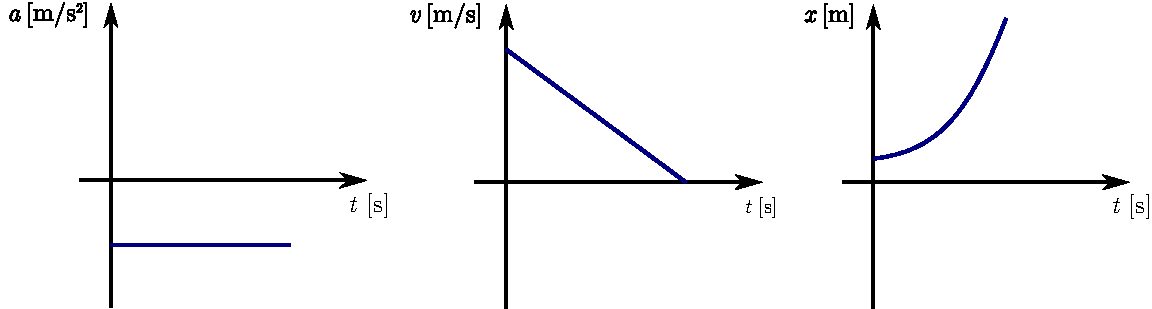
\includegraphics[width=0.8\textwidth]{img/prob11.pdf}
      \caption{\label{fig:prob11} Problema \ref{prob:11}}
  \end{figure}
    

\item \label{prob:12} La gráfica de la Figura~\ref{fig:prob12} corresponde a la velocidad en función del tiempo de un movimiento rectilíneo.
  
  \begin{figure}[!htb]
    \centering
    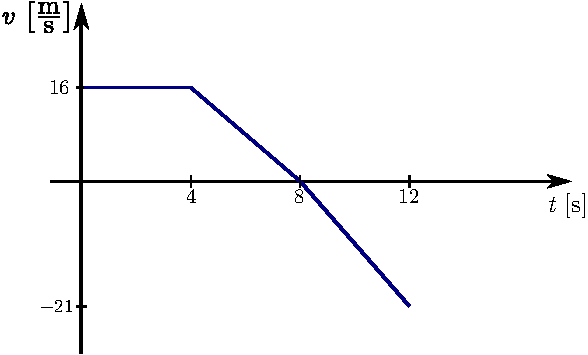
\includegraphics[scale=0.8]{img/prob12.pdf}
    \caption{\label{fig:prob12} Problema \ref{prob:12}}
  \end{figure}
  
  Calcula:
  \begin{enumerate}
    \item Distancia recorrida y valor del desplazamiento a los 12\,s.
    \item Velocidad media en [0; 12]\,s.
    \item Velocidad a los 5\,s.
  \end{enumerate}
  Grafica:
  \begin{enumerate}
    \item $a =  a(t)$ en [0; 12]\,s.
    \item $x =  x(t)$ en [0; 12]\,s.
  \end{enumerate}

  \resp{a) $Dist|_{t\,=\,12\,s} =  138$\,m y $\Delta \bar{x} \ = $ \{horizontal, hacia la derecha, 54\,m\}; \, b) $\bar{v}_m\ = $ \{horizontal, hacia la derecha, 4,5\,m/s\};\, c) $\bar{v}(5\,s)\ = $ \{horizontal, hacia la derecha, 12\,m/s\}.}

  \item Un vehículo viaja a 90\,km/h cuando el conductor ve un animal en la carretera 40\,m adelante. Si el tiempo de reacción del conductor es de 0,48\,s (aplica los frenos 0,48\,s después de ver el animal), y la desaceleración máxima de los frenos es de 7,6\,m/s$^2$ ¿El automóvil se detendrá antes de chocar al animal?
  
  \item Un electrón tiene una velocidad inicial de $3 \times 10^5$\,m/s. Si experimenta una aceleración de $8 \times 10^{14}$\,m/s$^2$, ¿cuánto tardará en alcanzar una velocidad de $5.4 \times 10^5$\,m/s? y ¿qué distancia recorre en este tiempo?
  \resp{$t  =  3 \times 10^{-10}$\,s; $Dist  =  1.26 \times 10^{-4}$\,m.}

  \item Dos amigos se ven cuando están a una distancia de 160\,m y corren a encontrarse. Uno corre a 10\,m/s y el otro a 7,5\,m/s. ¿Qué distancia recorre cada uno hasta encontrarse?
\resp{$Dist_{A1} =  91,43$\,m; $Dist_{A2} =  68,57$\,m}

  \item Un auto marcha a una velocidad de 80\,km/h en una zona escolar. Un coche de policía se pone en marcha en el momento en que el auto pasa junto a él y acelera de un modo constante a razón de 8\,km/h-s (2,2\,m/s$^2$).
  \begin{enumerate}[label=\alph*)]
  \item Grafica $x$ vs. $t$ para ambos coches.
    \item ¿Cuándo alcanza el coche de policía al auto?
    \item ¿Con qué rapidez irá el coche de policía en ese momento?
  \end{enumerate}
   \resp{b) $t_{encuentro} =  20$\,s; c) $|\bar{v}_{encuentro}|\ = $ 160\,km/h.}

  \item
  \begin{enumerate}
    \item Un automóvil frena hasta detenerse con una desaceleración uniforme $a$ en un tiempo $t$. demuestre que la distancia recorrida durante ese tiempo está dada por $\displaystyle x =  \frac{v^2}{2a}$  donde $v$ es la velocidad inicial y la dirección positiva se toma en sentido del movimiento inicial.
    \item Si  su velocidad inicial es de 90\,km/h y su aceleración es 5\,m/s$^2$, ¿qué distancia recorre hasta detenerse?
    \item Si ahora la velocidad inicial es de 180\,km/h, calcule la nueva distancia de frenado y compare con el valor anterior (es mayor o menor, es el doble, el triple, etc.)
    \item A partir de la expresión obtenida en a), trate de deducir qué ocurre con la distancia de frenado cuando se duplica la velocidad inicial.
  \end{enumerate}

  \item Un electrón en un tubo de rayos catódicos de un televisor entra en una región con velocidad $v_0$ y acelera de manera uniforme hasta una rapidez $v$ en una distancia $d$. Si la dirección del movimiento es a lo largo del eje x.
  \begin{enumerate}
    \item Demuestre que la expresión para calcular el tiempo que el electrón está en la región donde se acelera es $\displaystyle t =  \frac{2 d}{v_0 \ + \ v}$.
    \item Si la velocidad inicial del electrón es de $3 \times 10^4$\,m/s, su velocidad final es de $5 \times 10^6$\,m/s y recorre una distancia de 2\,cm. ¿Durante cuánto tiempo el electrón se acelera?
  \end{enumerate}

  \item Juan y Ana hicieron un viaje de Rosario a Santa Fe. Ana fue la mitad de la distancia a velocidad $v_1$ y la otra mitad a velocidad $v_2$. Juan en cambio, fue la mitad del tiempo a velocidad $v_1$ y la otra mitad a velocidad $v_2$. Si $v_1 =  2\,v_2$ y los dos salieron juntos de Rosario ¿Quién llegó antes? ¿Por qué?

  \item Una persona camina a través de una habitación de tal modo que, después de haber iniciado el movimiento, su velocidad es negativa pero su aceleración es positiva.
  \begin{enumerate}
    \item ¿Cómo sigue esto?
    \item Realiza un gráfico $v =  v(t)$ para este movimiento.
  \end{enumerate}
\end{enumerate}


\begin{thebibliography}{99}
\bibitem{f0} {``Física 1''; Maiztegui A P, Sábato J, Kapelusz; 2da ed., Buenos Aires, 2005}
\bibitem{01} {``Movimiento en una dimensión''; Grigioni L, Palmegiani M, Schafir A; Instituto Politécnico Superior, UNR, Rosario, 2017}
  \bibitem{02} {``Física''; M. Alonso, E. J. Finn; Addison--Wesley Iberoamericana, Estados Unidos,1995}
  \bibitem{f1} {``Física''; Wilson J, Buffa A, Lou B; Prentice Hall Inc., México, 2007}
  \bibitem{f2} {``Física para la Ciencia y la Tecnología''; Volumen 1; Tipler P, Editorial Reverté, España, 2001}
  \bibitem{f3} {``Fundamentos de Física'', Volumen 1; Serway R, Faughn J; 6ta ed., International Thomson Editores, México, 2004}
  \bibitem{f4} {``Física. Conceptos y aplicaciones''; Tippens P; Mc Graw Hill, México, 2001}
  \bibitem{f5} {``Física''; Wilson J; Prentice Hall Hispanoamericana, México, 1996}
  \bibitem{f6} {``Física''; Blatt F; Prentice Hall Hispanoamericana, México, 1991}
  \bibitem{f7} {``Física'', Tomo 1; Serway R; Mc Graw Hill, México, 1997}
  \bibitem{f8} {``Física. Principios y aplicaciones''; Giancoli D; Editorial Reverté, España, 1985}
  \bibitem{f9} {``Física EGB 3''; Reynoso L; Editorial Plus Ultra, Brasil, 1998}
  \bibitem{f10} {``Física General''; Alvarenga B,  Máximo A; Editorial Harla, México, 1981}
  \end{thebibliography}
  \thispagestyle{empty}


%\end{document}
